In questo capitolo si definiscono le specifiche di progettazione del servizio di visualizzazione dei trasporti pubblici, iniziando con un'introduzione al diagramma delle classi di progetto e l'adattamento del diagramma del modello di dominio concepito nel capitolo precedente ad un punto di vista software.

%%%
%%%possibile introduzione ai frameworks
%%%


\section{Diagramma delle Classi di Progetto} % (fold)
\label{sec:diagramma_delle_classi_di_progetto}

Nel capitolo precedente è stato definito il diagramma del modello di dominio, che rappresenta da un punto di vista grafico le classi concettuali presenti nella realtà di interesse di questa tesi. Esso quindi non rappresenta una modellazione tecnica da poter utilizzare in fase di progettazione, ma si limita a rappresentare in maniera semplice ed essenziale le proprietà e i concetti fondamentali dell'ambiente in studio.
Vi è bisogno dunque di compiere un'ulteriore passo in avanti verso un punto di vista di sviluppo applicativo, rimodellando le classi concettuali del modello di dominio in classi e oggetti software.

Per fare questo, viene utilizzato il diagramma delle classi di progetto, o DCD, il quale scopo è rappresentare in modo dettagliato le classi software, variabili e relazioni così da permettere uno sviluppo efficiente e garantisce una bassa presenza di reiterazioni in fase di implementazione.
% section diagramma_delle_classi_di_progetto (end)

\section{Struttura del DCD} % (fold)
\label{sec:struttura_del_dcd}

Il diagramma delle classi sfoggia una struttura per molti aspetti simile al diagramma del modello di dominio. Essendo una forma avanzata del modello di dominio questo aspetto risulta ovvio, ma dovendosi avvicinare ad una visione orientata puramente allo sviluppo software vi è il bisogno di definire ulteriori dettagli indispensabili nella fase di implementazione.

Seguirà ora una breve descrizione di come gli elementi del modello di dominio siano adattati sotto nuove forme nel diagramma delle classi di progetto.

\subsection{Classificatore} % (fold)
\label{sub:classificatore}

Per quanto riguarda le classi concettuali del modello di dominio, nel diagramma delle classi esse vengono rappresentate attraverso {\itshape classificatori}: un classificatore è un elemento di modello che descrive caratteristiche comportamentali e strutturali. Nel diagramma delle classi i classificatori possono identificare classi regolari o interfacce.

Ogni classificatore dispone inoltre di uno o più attributi o metodi, i quali permettono la conoscenza e l'interazione tra altri classificcatori presenti nel diagramma delle classi.
% subsection classificatore (end)

\subsection{Attributi} % (fold)
\label{sub:attributi_dcd}
Gli attributi di un classificatore sono mostrati in due modi. Essi possono essere elencati all'interno del classificatore, proprio come accade nel modello di dominio, rappresentando così dei contenuti informativi del classificatore.

Nel caso un classificatore abbia un attributo che faccia riferimento ad un'altro classificatore, viene utilizzato l'attributo tramite linea di associazione. Come nel diagramma del modello di dominio, le linee di associazione dispongono di una molteplicità, mentre il verso di percorrenza non è più bidirezionale, ma è orientato verso il classificatore a cui l'origine dell'associazione fa riferimento. Se un oggetto software contiene una collezione di attributi la molteplicità dell'associazione sarà dunque N, od 1 se il riferimento è singolo.
% subsection attributi (end)

\subsection{Operazioni} % (fold)
\label{sub:operazioni}
All'interno del classificatore risiede inoltre un'altra sezione adibita alle {\itshape operazioni}. Nel linguaggio UML, un'operazione è una dichiarazione costituita da nome, parametri e un tipo di valore di ritorno. Inoltre un'operazione può possedere un numero di vincoli che deve soddisfare per essere eseguita.

L'operazione tuttavia non è un metodo, in quanto l'operazione non definisce un'implementazione. Per quella fase si utilizzano per l'appunto i metodi, i quali implementano le operazioni descritte nel diagramma delle classi.
% subsection operazioni (end)

% section struttura_del_dcd (end)

\section{DCD: servizio di visualizzazione dei trasporti} % (fold)
\label{sec:dcd_servizio_di_visualizzazione_dei_trasporti}

Avendo dunque introdotto i concetti e le proprietà del diagramma delle classi di progetto, il prossimo passo è dunque rimodellare il modello di dominio definito nel capitolo precedente in un DCD di elevata fedeltà.

Prendendo dunque come riferimento il modello di dominio, il diagramma delle classi dispone di quattro classificatori principali:\\

{\itshape Linea}

{\itshape Direzione}

{\itshape Fermata}

{\itshape Autobus}\\

Concependo come classi regolari questi quattro oggetti, si prosegue assegnando ad ognuno gli attributi di riferimento e le dipendenze, giungendo ad un diagramma illustrato nella prossima pagina:
\newpage
\vspace{1cm}
\begin{figure}[htbp]
\begin{center}
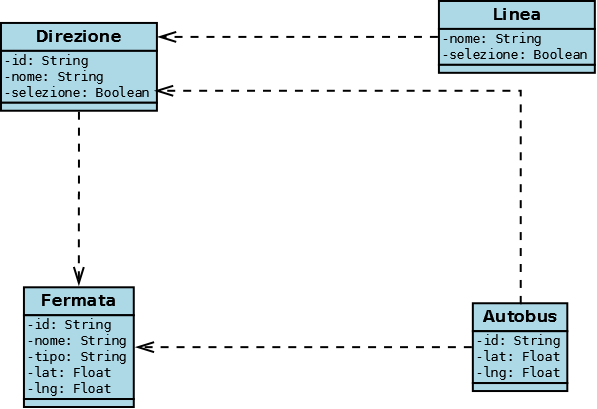
\includegraphics[width=10cm]{contents/images/dcd1}
\end{center}
\caption{Primo diagramma delle classi}
\label{fig:dcd}
\end{figure}
\vspace{1cm}
La classe Linea dispone di un attributo ``nome'' di tipo stringa, ed esso, come nel modello di dominio, assume un ruolo di identificatore nella collezione di oggetti linea che si vuole monitorare.
a Direzione è costituita da un attributo ``id'' e ``nome'', l'id sarà presente anche nelle classi successive, ed è quello che identificherà univocamente le istanze degli oggetti, assegnando invece al nome un contenuto puramente informativo, data la sua eccessiva lunghezza.
Nelle classi Fermata e Autobus sono presenti gli attributi ``latitudine'' e ``longitudine'', i quali definiscono la posizione univoca dell'oggetto nello spazio. Ciò permette la locazione di questi elementi durante la fase di posizionamento sulla mappa di visualizzazione.
Si può notare che le classi Direzione e Linea contiene un attributo ``selezione'', il quale sarà di utilità durante l'implementazione e lo sviluppo, in quanto permette di conoscere le linee e direzioni di preferenza dell'utente.
Infine è stato aggiunto l'attributo ``tipo'' nella classe Fermata, che permette di distinguere una fermata capolinea di partenza, capolinea di arrivo o semplice fermata d'intermezzo.

Per quanto riguarda le dipendenze, la classe Linea ne specifica una verso Direzione, in quanto ogni linea è costituita dalle sue direzioni. Per lo stesso motivo la classe Direzione dispone di una dipendenza verso Fermata. Concludendo con la classe Autobus, esso deve essere assegnato ad una direzione e inoltre deve collocarsi su una fermata, perciò avrà due dipendenze verso le rispettive classi.

Questa prima iterazione del diagramma delle classi di progetto non è però soddisfacente ai fini di sviluppo di un'applicazione web lato client, e deve dunque essere migliorato attraverso l'aggiunta di ulteriori classi che si occupino della gestione delle richieste, il prelievo dei dati, la manipolazione e la visualizzazione di questi ultimi attraverso un'interfaccia.

Possiamo dunque introdurre una classe {\itshape Applicazione}, che sarà la basedia del progetto. Questa classe si occupa di gestire tutte le altre classi e mantenerne i riferimenti.
L'applicazione, per quanto classe {\itshape madre} dell'intero sistema, non deve assurmersi altre responsabilità, come la gestione dei dati e delle richieste degli utenti, in modo da non caricare troppo il suo margine di compiti.

E' opportuno quindi definire una classe {\itshape Controller}. Il compito dell'entità Controller è la cattura e gestione delle richieste che l'utente pone al sito web. Inoltre si occupa della richiesta al server dei dati di interesse all'utente e della loro manipolazione, in modo che siano pronti per una corretta visualizzazione.

Proprio per quest'ultimo aspetto vi è il bisogno di creare una classe {\itshape Vista}, la quale fa riferimento alle classi di dati gestite dal sistema e si occupa della loro visualizzazione ad ogni nuova richiesta e, quindi, cambiamento del set di dati da dover visualizzare.
\newpage
Al seguito di queste nuove scelte progettuali, il nuovo diagramma delle classi assume la forma seguente:

\vspace{1cm}
\begin{figure}[htbp]
\begin{center}
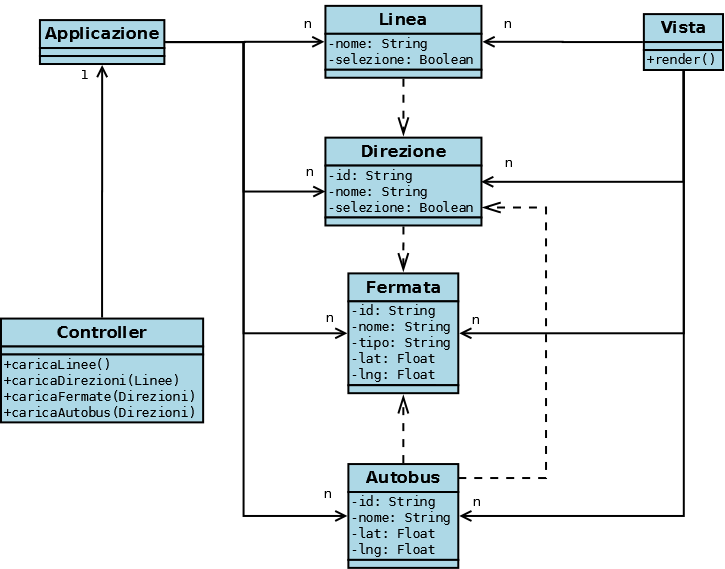
\includegraphics[width=13cm]{contents/images/dcd2}
\end{center}
\caption{Secondo diagramma delle classi}
\label{fig:placeholder}
\end{figure}
\vspace{1cm}

La classe Applicazione, dovendo mantenere dei riferimenti verso le altre classi, dispone di attributi per associazione verso tutte le altre classi definite nel diagramma. Le associazioni verso le classi Linea, Direzione, Fermata e Autobus saranno 1 a N, essendo quest'ultime collezioni di dati di interesse.

La classe Controller dipone di un riferimento verso l'Applicazione, potendo così attingere alle classi di dati e poterle manipolare. Essa dispone dei metodi CaricaLinee(), CaricaDirezioni(linee), CaricaFermate(direzioni) e CaricaAutobus(direzioni), i quali inoltrano una richiesta al server per ottenere i dati di interesse da immagazzinare in modo temporaneo nel client.

\newpage
La classe Vista sarà dotata di riferimenti verso le classi di dati Linea, Direzione, Fermata e Autobus, ed è costituita da un metodo Render(). Questo metodo permette la visualizzazione dei dati prelevati dal server ed immagazinati nel client, dove ognuno disporrà di uno stile di visualizzazione adatto.\\

Attraverso quest'ultima iterazione del diagramma delle classi, si è definito un sistema esaustivo per la creazione di una web application, nei capitoli successivi si descriveranno le scelte progettuali dei framework per lo sviluppo dello struttura lato client e le scelte per la realizzazione dell'interfaccia grafica.

\newpage
% section dcd_servizio_di_visualizzazione_dei_trasporti (end)